\documentclass{osudissert96}
\usepackage{natbib}

% BibTeX from the BiBTeX Documentation
\def\BibTeX{{\rm B\kern-.05em{\sc i\kern-.025em b}\kern-.08em
    T\kern-.1667em\lower.7ex\hbox{E}\kern-.125emX}}

%
% It is better to break up the dissertation into multiple files (e.g.,
% one file per chapter, as well as separate files for the abstract,
% acknowledgements, and vita).  These files are brought into the
% document using \include{} statements.  There will be times, however,
% when you don't want to print the ENTIRE dissertation.  You can limit
% what will actually be printed by using the \includeonly{} statment.
% This contains a list of the files you want printed.  Any file NOT
% listed will not be printed.  However, all page numbers, references,
% etc., will be preserved as though all the files were actually
% printed. For example, the line below would result only in chapters 1
% and 3 being printed (if it were uncommented).
%

%\includeonly{ch_introduction}

% UPDATED TEXT (2010):
%  In the newest format, titles should be title case everywhere.
%
% HISTORICAL TEXT (1996):
%  In the new format, the titles of each chapter should appear in
%  uppercase.  In the TOC, however, they should be in lowercase.
%  The command below automates this behavior.  However, you'll have to be
%  careful not to include \labels within your \chapter definitions or
%  there will be problems.  If you don't want this to be automated, comment
%  out the \typesetChapterTitle definition below and do your chapters in
%  the form:
%  \chapter[MY TITLE]{My Title}
%
%  \renewcommand\typesetChapterTitle[1]{\uppercase{#1}}
\renewcommand\typesetChapterTitle[1]{#1}

\begin{document}

%
% First, declare the parts of your title page 
%

\author{Michael Crawley}
\title{Understanding the Aeroacoustic Radiation Sources and Mechanism in High-Speed Jets}
\authordegrees{B.S.}  % Degrees thus far, not including this one.
\unit{Department of Mechanical Engineering}

\advisorname{Mo Samimy}
\member{Datta Gaitonde}
\member{James Gregory}
\member{Mei Zhuang}      % Normally you will have advisor + 2 members


%
% The following creates the title page
%

\maketitle
\disscopyright


%
% Abstract goes here.
%

\begin{abstract}
  %  The dissertation abstract can only be 500 words.
It has been well-known within the aeroacoustic community that the dominant noise sources in high-speed turbulent jets are related to the large-scale structures which are generated in the initial shear layer by instabilities and which rapidly grow as they convect downstream.
However, the exact dynamics of these large-scale structures which are relevant to the noise generation process are less clear.
This work represents an attempt to study the dynamics and noise generated by the large-scale structures quantitatively and in high-fidelity in a Mach 0.9 turbulent jet using simultaneous pressure and velocity data acquisition systems alongside plasma-based excitation to produce coherent ring vortices in the shear layer.

In the first phase, the irrotational near-field pressure is decomposed into its constitutive acoustic and hydrodynamic components, and two-point cross-correlations are used between the acoustic near-field and far-field in order to identify the dominant noise source region.
Building upon the work of previous researchers, the decomposition is performed using a spatio-temporal wavelet transform, which was found to be more robust than previous algorithms.
Results indicated that for both individual as well as periodic large-scale structures, the dominant noise source region constitutes the upstream region of the jet, ending just before of the end of the potential core (in a time-averaged sense) in the unexcited jet.

The large-scale structure interactions were then investigated by stochastically-estimating the time-resolved velocity fields from the time-resolved near-field pressure.
For computational efficiency, the ensemble velocity snapshots were first decomposed into orthogonal modes, and the a mapping from the near-field pressure to the expansion coefficients was then produced using a feedforward neural network using backpropagation for learning.
The coherent structures generated by the excitation were then identified and tracked using standard vortex identification routines.
For the impulsively-excited jet, the individual structures quickly rolled up into a coherent structure within two jet diameters and then advected until roughly four jet diameters downstream, at which point it underwent a rapid disintegration.
For the periodically-excited jet, multiple smaller-scale structures are initially produced; these quickly merge into a single large-scale structure which matches the excitation wavelength.
Similar to the impulsively-excited structures, these now large-scale structures advect downstream and undergo a rapid disintegration near the end of the potential core. 

Finally, from Ribner's dilatation-based acoustic analogy the aeroacoustic source terms were computed using the time-resolved velocity field produced by the stochastic estimation.
Interpretation of the results is limited however, due to the number of assumptions and simplifications necessary for the computations, given the realities of the available experimental facilities.
Analysis of the computed source fields identified the coherent structures producing a convected wavepacket-like event, centered on the jet lipline though reaching into the potential core.
For the individual vortex rings, a clear modulation of the spatial extent and amplitude was observed as the vortex began to break down just upstream of the end of the potential core.
This behavior is also present for the periodic train of vortices, however it is obscured by an amplification of the source in the upstream region, corresponding to the pairing location for the multiple smaller-scale structures generated by the excitation. 



\end{abstract}

\dedication{This work is dedicated to Science \ldots}


%
% Bring in Acknowledgement and Vita from separate files named ``ack.tex''
% and ``vita.tex''.
%

\begin{acknowledgements}
I should probably acknowledge someone here \ldots
\end{acknowledgements}


\begin{vita}

\dateitem{September 10, 1986}{Born - Plano, Texas}

\dateitem{2009}{B.S. Mechanical Engineering, \\
				University of Texas, Austin.}

\dateitem{2009-present}{Graduate Research Associate,\\
			 The Ohio State University.}


\begin{publist}

%% UPDATE FOR 2010:
%  Grad school only wants research publications, and it only wants those
%  research pubs that are actually published. Accepted or ``to appear''
%  publications don't count. If they look closely, they'll tell you to
%  remove any publications that aren't in print. Haivng said that, they
%  probably won't look that closely unless you put a really long list
%  here. You're tempting fate if you add instructional publications
%  though.

\researchpubs

\pubitem{\textbf{M. Crawley}, C.-W. Kuo, and M. Samimy,
\newblock ``Identification of the Acoustic Response in the Irrotational Near-field of an Excited Subsonic Jet.''
\newblock submitted to \emph{International Journal of Aeroacoustics}.}
	

\pubitem{\textbf{M. Crawley}, R. Speth, D. V. Gaitonde, and M. Samimy, 
\newblock ``A Study of the Noise Source Mechanisms in an Excited Mach 0.9 Jet - Complementary Experimental and Computational Analysis.''
\newblock AIAA Paper 2015-0736, \emph{53$^{rd}$ AIAA Aerospace Sciences Meeting}.}
	

\pubitem{\textbf{M. Crawley}, A. Sinha, and M. Samimy, 
\newblock ``Near-field and Acoustic Far-field Response of a High-Speed Jet Forced with Plasma Actuators.''
\newblock \emph{AIAA Journal}, expected 2015.}
	

\pubitem{\textbf{M. Crawley} and M. Samimy, 
\newblock ``Decomposition of the Near-Field Pressure in an Excited Subsonic Jet.''
\newblock AIAA Paper 2014-2342, \emph{20$^{th}$ AIAA/CEAS Aeroacoustics Conference}.}
	

\pubitem{\textbf{M. Crawley}, A. Sinha, and M. Samimy, 
\newblock ``Near-field Pressure and Far-field Acoustic Response of Forced High-Speed Jets.''
\newblock AIAA Paper 2014-0527, \emph{52$^{nd}$ AIAA Aerospace Sciences Meeting}.}	
	

\pubitem{\textbf{M. Crawley}, H. Alkandry, A. Sinha, and M. Samimy, 
\newblock ``Correlation of Irrotational Near-Field Pressure and Far-Field Acoustic in Forced High-Speed Jets.''
\newblock AIAA Paper 2013-2188, \emph{19$^{th}$ AIAA/CEAS Aeroacoustics Conference}.}
	

\pubitem{H. Alkandry, \textbf{M. Crawley}, A. Sinha, M. Kearney-Fischer, and M. Samimy,
\newblock ``An Investigation of the Irrotational Near Field of an Excited High-Speed Jet.''
\newblock AIAA Paper 2013-0325, \emph{51$^{st}$ AIAA Aerospace Sciences Meeting}.}
	

\pubitem{\textbf{M. Crawley}, M. Kearney-Fischer, and M. Samimy, 
\newblock ``Control of a Supersonic Rectangular Jet Using Plasma Actuators.''
\newblock AIAA Paper 2012-2211, \emph{18$^{th}$ AIAA/CEAS Aeroacoustics Conference}.}
\end{publist}



\begin{fieldsstudy}

% The \majorfield* uses the unit specified in the \unit command used
% earlier in your document. If you want to use a different unit, use the
% second form shown here
%\majorfield*
\majorfield{Mechanical and Aerospace Engineering}

%%
%% Note:  If there were only one field of study, the following list 
%%        would best be done using the following command:
%%
%%  \onestudy{Only Topic}{Only Professor}
%%

% \begin{studieslist}
% \studyitem{Topic 1}{Prof.\ Big Dude}
% \studyitem{Topic 2}{Prof.\ Other Dude}
% \studyitem{Topic 3}{Prof.\ Another Dude}
% \end{studieslist}

\end{fieldsstudy}

\end{vita}




%
% Make the Table of Contents and other good stuff
%

\tableofcontents
\listoftables
\listoffigures


%
% The following is a list of chapters.  Each is brought in from a
% separate file using the \include{} command.
%

\chapter{Introduction}
\label{introduction}
\section{Motivation}
The advent of the turbojet engine led to a transformation in both commercial and military aviation, allowing for much faster flight than previously possible with propellor-driven aircraft. 
However, the increased thrust of turbojets has come at great cost; significant acoustic radiation is generated by the rotating components (compressor, turbine, fan), by the combustion process, and ultimately by the free jet itself. 
On the commercial side, the escalating number of flights, encroachment of urban and residential areas near airports, and tightening of environmental regulations have combined to force airports to institute curfews, surcharges and flight path restrictions to combat noise pollution. 
For the military, hearing damage inflicted on nearby personnel (particularly flight deck crew on aircraft carriers) has necessitated the implementation of noise reduction concepts on tactical aircraft.
During takeoff and landing, when acoustic radiation is most problematic to ground crew and  surrounding urban and residential areas, the dominant noise source of the jet engine is the aeroacoustic radiation generated by the high velocity engine exhaust.
This has spurred extensive research, spanning over six decades, into the acoustic source mechanism in high speed, high Reynolds number jets. 

While progress has been made in the field of aeroacoustics, both experimentally \citep{Tam1996, Viswanathan2006, Tam2008} as well as theoretically \citep{Cabana2008}, understanding of jet noise sources and their radiation mechanisms remains incomplete \citep{Jordan2008}.
This is due to the large number of interrelated parameters (e.g. Reynolds number, temperature ratio, acoustic Mach number, nozzle geometry, et cetera) as well as the large disparity in the associated length and time scales of the turbulent phenomena and the radiated noise.
Simulations of controlled free shear layers have suggested that there is significant potential for noise reduction, on the order of 11 dB in some cases [Wei 2006].
However, these simulations relied on non-physically defined actuation (that is, forcing was applied over a defined region by arbitrary energy, momentum, and body force terms), and a physical interpretation of the optimum forcing parameters was not immediately clear to the researchers.
Current noise-mitigation technologies for free jets have largely been applied in an adhoc fashion, due to our incomplete understanding of the aeroacoustic sources.
Fully realizing this maximum noise reduction potential will require a much more detailed understanding of the mechanism (or mechanisms) by which free jets radiate to the far-field.

It is generally agreed that the dominant noise sources are related to the large-scale turbulent structures present in the mixing layer of the jet. 
What remains to be determined is what aspects of the large-scale structure evolution and interactions are relevant to the noise generation process. 
Theoretical models of spatially- and temporally-modulated coherent structures have shown great promise in replicating the observed characteristics of the dominant far-field noise [Cavalieri/Jordan?]. 
However, direct experimental data linking this structure evolution to the acoustic emission is still lacking. 
It is on this vein that the current work is focused.
Until recently, experimental data acquisition techniques have been unable to capture the flow physics with enough fidelity (lacking in either spatial or temporal resolution) in order to accurately model the large-scale structures and aeroacoustic sources.
By combining contemporary data acquisition methods (free-field microphones and non-time-resolved particle image velocimetry) with novel post-processing algorithms this work aims to directly link the relevant vortex dynamics of the large-scale structures to the acoustic emission events, and in the process identify a simplified aeroacoustic source mechanism. 

This study can be broken down into three distinct parts. 
In the first, the irrotational near-field and acoustic far-field of the jet is analyzed in order to identify the dominant acoustic source region.
In the second, time-resolved velocity fields are estimated using an artificial neural network, which is trained to generate a mapping from time-resolved pressure measurements to instantaneous velocity.
Lastly, the acoustic source is computed from the time-resolved velocity using Ribner's simplification of Lighthill's acoustic analogy.  
	
\section{Background}
\subsection{Flow Control}
\label{sec:flow_instabilities}
Controlling the development of the jet plume, and hence controlling the rate of mixing or intensity and characteristics of the emitted acoustic radiation, is a long running goal of the aeroacoustic community.
Passive, permanent modifications to the nozzle have been shown to be quite adept at this task; some examples of these include tabs [citations] and chevrons [citations]. 
These work to generate counter-rotating streamwise vortices in the developing shear layer, which serve to substantially increase mixing between the core and coflow in the near-nozzle region and ultimately retard the growth of large-scale axisymmetric structures [citation].

Unfortunately, these passive modifications have associated penalties to the engine performance, in terms of added weight or reduced thrust.
Due to the passive nature of the flow modification, these performance penalties are in effect over the entire duration of the flight regardless of whether or not the noise reduction is needed. 
To improve engine efficiency, active control techniques are desired, since they can be activated when needed, such as during takeoff and landing, and deactivated when unneeded, such as after a commercial airliner reaches cruising altitude. 
Active control techniques, which seek to manipulate instabilities in the jet shear layer, have been extensively studied in low-speed, low-Reynolds number jets, the most common of which is acoustic drivers [citations]. 
However, as the speed and Reynolds number of the jet is increased (to match those in practical applications), so too does the required bandwidth and energy of the active drivers. 
Hence, acoustic or magneto-hydrodynamic drivers lose control authority in these regimes, and more powerful actuators are required.

The last decade has seen a rapid growth in the development of plasma actuators for use in high-speed flow control; though as of yet they have not progressed past the experimental phase.
Localized arc filament plasma actuators (LAFPAs) are one such class of plasma actuator, which were developed by a collaboration between the Gas Dynamics and Turbulence Laboratory (GDTL) and the Non-Equilibrium Thermodynamics Laboratory (NETL) at the Ohio State University.
LAFPAs can provide the high-amplitude and high-frequency excitation required for control of high Mach number and high Reynolds number jets [citations]. 
GDTL has used these actuators for noise mitigation and flow control in Mach 0.9 [citations], Mach 1.3 [citations] and Mach 1.65 [citations] jets (both heated and unheated). 
A review of the development of LAFPAs and their use in flow control and fluid phenomena research in high speed, high Reynolds number jets can be found in Samimy et al. [citation]. 
More recently, the diagnostic potential of LAFPAs for understanding jet flow phenomena has been explored. Excitation of instabilities in the flow by LAFPAs results in a definitive spatio-temporal origin to which resulting phenomena can be referenced. 
The absolute temporal reference afforded by LAFPA excitation provides researchers the ability to investigate the growth, saturation, and decay of structures with high fidelity. 
An example of their diagnostic potential can be found in the work of Kearney-Fischer \etal [citation], which investigated Mach wave radiation from heated, high Mach number jets using schlieren imaging phase-locked to LAFPAs. 

Unlike their passive counterparts (such as tabs or mechanical chevrons), or some other potential active flow control technologies (such as fluidic chevrons), LAFPAs control the shear layer development indirectly by exciting naturally occurring instabilities.
The sharp velocity gradient in the jet shear layer (or, more precisely the inflection point produced by this sharp gradient) gives rise to the inviscid Kelvin-Helmholtz instability [citation] (sometimes simply referred to as the initial shear layer instability).
This instability is broadband and scales with the local momentum layer thickness and jet exit velocity ($\theta / U_j$) ; perturbations over a wide range of frequencies can be amplified, though the dominant frequencies are found to be on the order of $St_{\theta} = f \theta /U_j = 0.012$ for very thin boundary layers [Cohen and Wygnasnki?]. 
The Kelvin-Helmholtz instability then drives the development of the large-scale structures in the shear layer by amplifying fine-scale perturbations, ultimately causing them to roll-up into coherent structures regardless of Reynolds number [Crow and Champaign, Brown and Roschko].
Owing to the axisymmetry of the jet nozzle (i.e. that the initial shear layer wraps around and connects to itself), various azimuthal Fourier modes are unstable to perturbations (including both axisymmetric and higher order modes) [Cohen?].

The growth of the shear layer as it advects downstream ultimately dictates that the shear layer merges with itself; this location is referred to as the end of the potential core.
A secondary instability, the jet column instability, manifests in axisymmetric jets and is related to the passage of large-scale structures through the end of the potential core.
This instability scales with the jet exit diameter and jet exit velocity ($D / U_j$) and is broadband, with a dominant characteristic frequency of $St_{D} = f D /U_j = 0.3$.
The relation of the jet column instability to the initial shear layer instability is not well understood.  
Kibens argued that the jet preferred frequency is related to the initial shear layer frequency by the number of pairings of large scale structures that occur before the end of the potential core (i.e. $f_n / f_p = 2^n$), as the frequency of the structures halves after each pairing process [Kibens].  
Conversely, Petersen claims that the jet preferred mode is simply the initial shear layer instability at the end of the potential core, and that the appearance of a single dominant lengthscale for the axisymmetric mode is due not to a type of `global' instability of the flow field, but to a cutoff at the end of the potential core of the axisymmetric instability [Petersen and Samet 1988].
Regardless, it is clear that the large-scale oscillations of the jet shear layer and potential core are ultimately the product of small-scale perturbations which are amplified by the initial shear layer instability.

LAFPAs achieve flow control by utilizing this relationship between the initial shear layer instability and the jet column instability.
The localized plasma arc-filament produces a rapid, localized heating through the Joule effect, and a compression wave is formed [Utkin 2007].
Though these perturbations are spatially discrete, they quickly amplify into large-scale coherent structures with well-defined characteristic spatial, temporal, and azimuthal frequencies.
Thus, LAFPAs are able to control the development of the most energetic scales in the jet shear layer; large-scale, azimuthally-coherent structures can be generated when enhanced mixing and jet spreading are desired, or smaller-scale, less azimuthally-coherent structures when noise reduction is necessary. 
In the present work, the subsonic jet is excited by LAFPAs, though here the goal is diagnostic rather than immediate practical application.
The well-defined frequencies and phase of the large-scale structures produced by LAFPA actuation serve as an excellent reference for data acquisition and post-processing (e.g. phase-locking and phase-averaging).

\subsection{Lighthill's Acoustic Analogy}
Far outside the jet, where the medium is quiescent, no sources or sinks are present, and any disturbances are low-amplitude and isentropic, the governing equations can be linearized and simply reduced to a homogeneous wave equation
\begin{equation}
	\frac{\partial^2 p}{\partial t^2} - c^2 \nabla ^2 p = 0
\end{equation}
which describes the non-dispersive propagation of (acoustic) waves through space and time.
Lighthill \citep{Lighthill1952} was the first to identify that the governing equations for fluid dynamics could also be rearranged in such a manner as to produce a propagating wave equation \textit{inside the jet}.
Prior to this, aeroacoustic studies had observed that the frequency content of the far acoustic field matched that of the flow field, but had not identified a way to estimate the acoustic intensity.

Starting with the conservation of mass and momentum equations, one can take the divergence of the former and the partial derivative with respect to time of the latter, and combine these along with the equation of state to produce
\begin{equation}
\frac{1}{c^2}\frac{\partial^2 p}{\partial t^2} - \nabla^2 p = \nabla \cdot \nabla \cdot \mathbf{T}.
\end{equation}
$\mathbf{T}$, commonly referred to as \textit{Lighthill's stress tensor}, comprises Reynolds stresses, viscous stresses, and entropy fluctuations, respectively:
\begin{equation}
\mathbf{T} = \rho \mathbf{u} \otimes \mathbf{u} - \mathbf{\tau} + \mathbf{I} \left[ (p-\bar{p}) - c^2 (\rho - \bar{\rho}) \right].
\end{equation}
Here, $c$ refers to the ambient speed of sound, $\mathbf{I}$ is the identity matrix, $\mathbf{\tau}$ is the shear stress tensor, and an overbar ($\bar{\cdot}$) corresponds to a time-averaged quantity.
This transformation has the effect of approximating the real system as a uniform acoustic medium at rest which is being driven by an external fluctuating force field.
As the wave operator is linear, the solution to this equation can be formulated with the aid of Green's functions,
\begin{eqnarray}
\frac{\partial^2 G}{\partial t^2} - c^2 \nabla^2 G = \delta (\tau -t) \delta (\mathbf{x}' - \mathbf{x}).
\end{eqnarray}
The solution to this (see Crighton \etal [cite]) is the deceptively simple spatial integration of the source field at retarded time (that is, it is accounting for the propagation delay from the source location to the observer):
\begin{equation}
p (\mathbf{x},t) = \frac{1}{4 \pi c^2} \nabla \cdot \nabla \cdot \int_{\Omega} \frac{\mathbf{T} (\mathbf{x}',t - |\mathbf{x} - \mathbf{x}'|/c)}{|\mathbf{x} - \mathbf{x}'|} d^3 \mathbf{x}'.
\end{equation}

Lighthill's derivation of what became known as the first acoustic analogy (which in fact was specifically tailored to the study of jet noise) reformed the study of aeroacoustics.
As has been discussed by many authors before (see Goldstein 1974 for example), this equation describes the propagation of sound, through a quiescent medium, generated by quadrupole sources. There have been several major assumptions made in this derivation, that the flow is completely subsonic (and hence no shock or expansion waves are present), that the observer location is far from the jet (and hence hydrodynamic pressure fluctuations or `pseudo-sound' is negligible), that there are no solid boundaries near the flow (and hence, no reflections, diffraction, absorption, or scattering) and finally that the acoustic waves themselves do not act as sources as they propagate through the flow.
Nonetheless, this theoretical framework is still applicable to a wide variety of commercial and scientific inquiries, present study included.

Theoretical work based on Lighthill's approach was successful in predicting some aspects of experimentally-observed jet noise.
Namely, stochastic source models of quadrupoles (per the aeroacoustic community's understanding of jet turbulence at the time) predicted a far-field pressure intensity scaling of $I \sim U_{j}^{8}$ which agreed with experimental results from cold, subsonic jets at sideline angles [Viswanathan].
However, this scaling law does not hold when the jet is heated, necessitating more complex source models. 
Unfortunately, given the complexity of the source field, even modern experimental techniques cannot acquire the full source with sufficient spatial and temporal fidelity to elucidate the flow structures responsible for the dominant noise emission.

Later researchers further refined Lighthill's approach (e.g. Howe [cite], Goldstein [cite] and Lilley [cite]); providing successively clearer characterizations of the source physics.
In addition to the true noise sources, Lighthill's acoustic source term includes flow-acoustic interactions, which describe diffraction and convection effects rather than true sources of noise, and which these researchers have attempted to separate from the true noise sources.
Alternative acoustic analogies have also been proposed, such as Powell's theory of vortex sound [cite] and Doak's momentum potential theory [cite].
In a slightly different vein, analytical decompositions have been performed in order to separate the disparate fluid phenomena inherent in Lighthill's source term and identify the roles of each [cabana 2008].
In each of these theories however, the source field for a high-speed, turbulent jet is highly complex and defies a simple physical understanding of the dynamical processes which lead to the noise emission.   

\subsection{The Role of Large-Scale Structures}
Initial understanding of turbulence was that it was stochastic in nature - that the frequency and appearance of turbulent eddies in a flow was random, with little to no prescribed preference.
It was in this context that Lighthill's acoustic analogy was first developed, and as a result initial models for the source field assumed a stochastic distribution of quadrupoles.
This source model was shown to produce an intensity which scaled with the eighth-power of the flow velocity, which was in general agreement with the experimentally-observed intensity scaling of cold, subsonic jets [Lighthill 1954].
The downstream convection of these quadrupoles produces a preferential directivity in the emitted acoustic radiation, with a maximum predicted to occur near 45$^\circ$ from the jet axis, again in general agreement of experimental far-field spectra [Lighthill 1954].
However, researchers have found that stochastic quadrupole source models fail to accurately predict the intensity scaling of jet noise in heated jets or cold jets at low observer angles [Tam 2008].
As Lighthill's analogy is an exact rearrangement of the governing equations (aside from the relatively minor assumption of a constant speed of sound), the error lies in our understanding of the aeroacoustic source. 

Mollo-Christensen [cite], and later Crow \& Champagne [cite] and Brown \& Roshko [cite], were the first to identified large-scale, coherent vortical structures underpinning turbulent free shear layers, in addition to the fine-scale, stochastic eddies.
Later researchers linked the appearance of these large-scale structures to natural flow instabilities (predominantly the Kelvin-Helmholtz instability discussed in \sect{sec:flow_instabilities}) [Michalke, Cohen and Wygnanski].
Following the identification these coherent structures in turbulent jet shear layers, source term models based on large-scale eddies have frequently been employed, to varying degrees of success. 

A simplified model of the noise generation process in stationary free jets can be found in \fig{fig:jet_sources_diagram}. 
This model is from the work of Tam \etal \citep{Tam1996, Tam2008}, who observed that the far-field spectra could be represented as a combination of two similarity spectra based on polar angle of the observer, regardless of jet Mach number or temperature.
At observer angles close to the jet downstream axis, the spectra exhibited a clearly defined spectral peak (\emph{F}-spectrum), whereas at sideline or upstream angles the spectra were broadband (\emph{G}-spectrum).
From this observation the two-component acoustic source model was born: the isotropic fine-scale turbulence, dominant in the near-nozzle region, is responsible for the omni-directional acoustic radiation that dominates the sideline and upstream polar angles. 
On the other hand, the large-scale turbulent structures which exist further downstream produce the superdirective radiation that is readily apparent at aft polar angles. 
This model of large-scale (and to a lesser extent fine-scale) turbulence noise generation explains the so-called 'mixing noise' generated by both subsonic and supersonic jets.
\begin{figure}
	\centering
	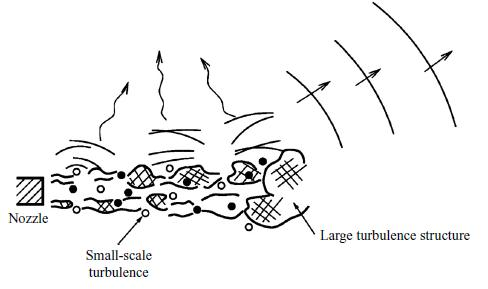
\includegraphics[width=5in]{Figures/JetNoiseSourceDiagramTMP.jpg}
	\caption{Simplified diagram of jet noise sources, reprinted from Tam \etal JFM 2008.}
	\label{fig:jet_sources_diagram}
\end{figure}
Numerous experimental studies have lent credibility to this view of aeroacoustic noise generation; see for example, Panda \etal [cite], Viswanathan \etal [cite], Tam \etal [cite], and Bogey \& Bailley [cite 2005].
There is little disagreement at this point that the large-scale coherent structures in the turbulent shear layer are responsible for the dominant noise emission; however, the exact dynamics of these which leads to acoustic emission are as of yet still not well-understood. 

[Wavepacket models???]
 
Additional noise source mechanisms have been identified for supersonic jets. In imperfectly expanded jets, shock cells are produced in the jet. As turbulent structures pass through these waves, the sharp pressure gradients cause them to emit acoustic radiation. 
This is observed directly in the far-field as a broad-band amplification at high frequencies, referred to simply as broad-band shock-associated noise (BBSAN). 
In stationary or subsonic airframes this radiation can generate a feedback loop, whereby the noise travels upstream to the nozzle exit, excites the initial shear layer, and produces new structures at the same frequency.
A high-amplitude, narrow-band tone (screech noise) is the end result of this feedback loop.
Lastly, supersonically-convecting (relative to the ambient) large-scale structures (which exist in supersonic and heated jets) produce high-amplitude, strongly-directional acoustic radiation towards aft angles.
This Mach wave radiation can be explained by a wavy-wall analogy [Tam].
In the present work, the jet is unheated and subsonic; as such these noise sources are not present and therefore neglected throughout the rest of this work.

      
\chapter{Background}
\label{background}
\section{Components of Jet Noise}

\section{Acoustic Analogy}

\section{Source Models}

\section{Flow Control}   
\chapter{Experimental Methodology}
\label{methodology}

\section{Anechoic Chamber}
All experiments were conducted at the GDTL within the Aerospace Research Center at the Ohio State University. 
Compressed, dried, and filtered air is supplied to the facility from two cylindrical storage tanks with a total capacity of 43 m$^{3}$ and maximum storage pressure of 16 MPa.
The air may be routed through a storage heater (not used in this study), which allows the jet to operate with a stagnation temperature up to 500 C, before expanding through a nozzle and exhausting horizontally into an anechoic chamber. 
Opposite the nozzle, a collector accumulates the jet and entrained air and exhausts to the outdoors. 
A schematic of the anechoic chamber can be seen in \fig{fig:chamber}. 
The dimensions of the chamber are 6.20 m wide by 5.59 m long and 3.36 m tall, with internal wedge-tip to wedge-tip dimensions of 5.14 m by 4.48 m and 2.53 m, respectively. 
The design of the chamber produces a cutoff frequency of 160 Hz, below the frequencies of interest for this study. 
A more detailed description of the GDTL anechoic chamber properties and validation has been given by [Hahn?].
\begin{figure}
	\centering
	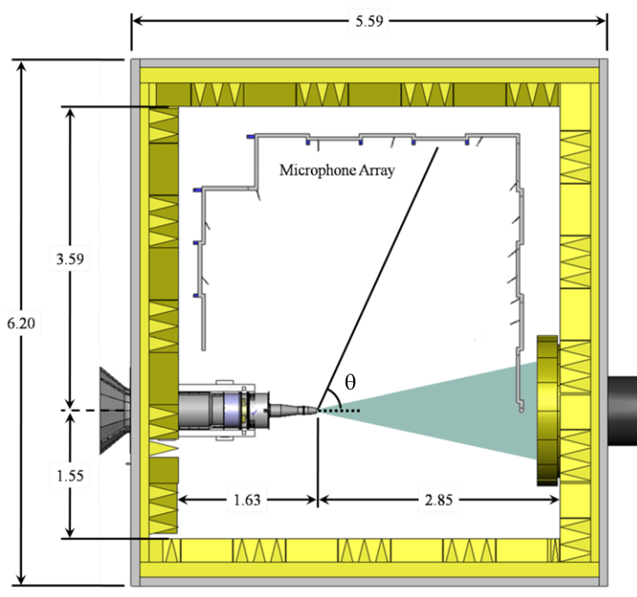
\includegraphics{Figures/Chamber_Schematic.png}
	\caption{Top-down view of anechoic chamber and free jet facility at GDTL; dimensions are in meters.} 
	\label{fig:chamber}
\end{figure}

For this study a converging, axisymmetric nozzle with exit diameter D of 25.4 mm was used. 
The internal contour of the nozzle was designed using a fifth order polynomial. 
The nozzle utilized a thick-lipped design in order to simplify the mounts for the LAFPA extension, which housed the eight actuators used in this study. 
For the experiments reported in this paper, the jet was operated at a Mach number ($M_j$) of 0.90, and with a total temperature ratio of approximately unity. 
The Reynolds number based on the jet exit diameter was $6.2\times〖10〗^5$; previous investigations using hot-wire anemometry have indicated that the initial shear layer is turbulent for this operating condition with momentum thickness ~0.09 mm and boundary layer thickness ~1 mm [Kearney?].

\section{Localized Arc-Filament Plasma Actuators}
The design of the localized arc-filament plasma actuators, as well as the driving circuitry, has undergone a slow evolution since their initial development by the GDTL and NETL.
In the current work, each LAFPA actuator consists of a pair of 1~mm diameter tungsten pin electrodes.
The center-to-center spacing between electrode pairs for each actuator is 4 mm.
Eight actuators were uniformly spaced around the nozzle perimeter 1 mm upstream of the nozzle exit. 
For electrical and thermal durability, the electrodes were housed in a boron nitride (grade AX05) extension attached to the end of the nozzle. 
A groove with dimensions of 1 mm wide and 0.5 mm deep is machined in the boron nitride, into which the electrode tips protrude, to provide a region of low momentum flow in order to stabilize the plasma arcs. 
It has been shown that the existence of this groove does not substantially alter the flow field or the control authority of the LAFPAs [citation]. 
A detailed description of initial development and LAFPA characteristics can be found in Utkin et al. [citation].

The LAFPAs were energized by a multi-channel, high-voltage plasma power generator ()capable of simultaneously powering up to eight LAFPAs), which was designed and built in-house at the GDTL. 
In the second-generation power supply, each individual circuit consists of a switchable capacitor in line with a high voltage transformer; the arcing electrodes are connected to the secondary side of the coil. 
The capacitor is charged by a 100 V DC power supply when the first switch is closed and the second is opened; at the user-specified time the switches flip and it discharges through the coil. 
The switches are controlled by a 16-channel digital I/O card and National Instruments' Labview software, operated by a dedicated computer. The plasma generator provides independent control of the frequency, duty cycle/pulse width, and phase of each individual actuator (though not the amplitude). 
The pulse width was held constant at 7 μs, which was found to be the minimum pulse width at which the actuators consistently arced for all frequencies explored in this study [citation]. 
The circuit is limited to 20 kHz due to thermal concerns.
However, as the current work is focused on the evolution of large-scale structures (and ultimately their acoustic radiation), this is not an issue.

\section{Data Acquisition}
\subsection{Near- and Far-field Pressure}
Near-field and far-field pressure measurements were acquired using Brüel \& Kjær ¼ inch 4939 microphones and preamplifiers. 
The signal from each microphone is band-pass filtered from 20 Hz to 100 kHz using a Brüel \& Kjær Nexus 2690 conditioning amplifier, and recorded using National Instruments PXI-6133 A/D boards and LabVIEW software. 
The microphones are calibrated using a Brüel \& Kjaer 114 dB, 1 kHz sine wave generator (model \# ???). 
The frequency response of the microphones is flat up to roughly 80 kHz, with the protective grid covers removed. 

Far-field acoustic pressure is acquired at three polar angles: 30°, 60° and 90°, as measured from the downstream jet axis. 
The positioning of the far-field microphone array can be seen in \fig{fig:chamber}.
The microphones were oriented such that they are at normal incidence to the jet downstream axis at the nozzle exit. 
The radial distance of the microphones ranges from 101D at 30° to 145D at 60°. 

The near-field pressure was acquired  during two separate experimental campaigns; the first focusing purely on the near-field and far-field pressure and the second focusing on the instantaneous velocity field. During the first campaign, the irrotational near-field was acquired using a linear array of sixteen microphones located along the meridional plane of the jet; the spacing varied along the array from 1D to 2D \fig{nearfield1_schematic}. 
The array was mounted on an x-y linear traverse system the array and was inclined at an angle of 8.6º to the jet axis in order to match the spreading angle of the jet shear layer, as determined via PIV measurements during previous studies [28]. 
The traverse was controlled using LabView and enabled the acquisition of pressure measurements at various radial positions with respect to the jet axis. 
Initially, the most upstream microphone is positioned at x/D = 1 and r/D = 1.20, which is just outside the initial shear layer.
For subsequent cases, the microphone array was incremented radially outward by 0.5D for a total travel distance of 7D, for a total of 15 array locations in the radial direction.
Voltage signals were collected at 200 kHz with 81920 data points per block; sub-blocks of 8192 data points were used when calculating short-time power spectral densities, resulting in a frequency resolution of 24.4 Hz. 
Ten blocks were recorded for each case resulting in four seconds of data, which has been found to be sufficient for statistical convergence.
\begin{figure}
	\centering
	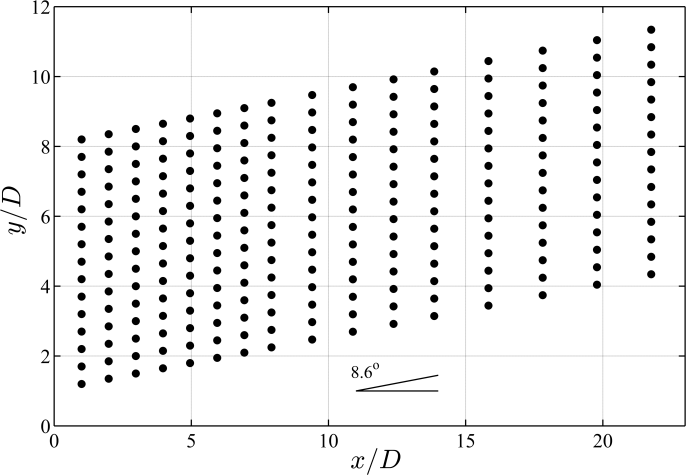
\includegraphics{Figures/NearField1_Schematic.png}
	\caption{Schematic of the microphone positions ???}
	\label{nearfield1_schematic}
\end{figure}

In the second experimental campaign, a shorter array consisting of 12 microphones equally space by $1D$ was used. 
In this case, the array was mounted from the floor and at an angle off the meridional plane of the jet (with microphone tips angled normal to the jet axis).
This setup was used in conjunction with the particle image velocimetry described in the following section; the microphone array was placed off of the meridional plane so that it did not intersect with the laser sheet. 
As before, the microphone array was angled 8.6º with respect to the jet axis in order to match the spreading rate of the shear layer, and the axial and radial position was set to match the closest microphone array location used during the first experimental campaign.
Voltage traces were acquired at 400 kHz, with 24576 points collected per block.
The voltage traces were collected simultaneously with streamwise particle image velocimetry measurements (described in the following section); 1500 blocks were acquired, corresponding to the 1500 acquired images.

In addition to the microphone voltage traces, the acoustics data acquisition system recorded a reference signal corresponding to the LAFPA excitation. 
The TTL pulse sequence, which controls the LAFPAs, was supplied to an Agilent 3320A waveform generator. 
The rising edge of the TTL pulse triggered a sharp drop in the output voltage of the waveform generator, which then ramps back up to the original voltage over a time interval which is shorter than the minimum excitation period. 
The output from the waveform generator was acquired simultaneously with the near- and far-field pressure signals using the aforementioned National Instruments hardware and software. 
As the excitation frequency, azimuthal mode, and ramp signal are well defined, this system enables the identification of the zero phase of actuation and hence, the ability to phase-average the pressure signals over the excitation period, akin to the work performed in Sinha et al [citation].
This ensures that the seeded perturbations can be readily identified in the noisy flow, as well as allowing pressure signals, which were not recorded simultaneously (i.e. different near-field array positions), to be analyzed concurrently. 

\subsection{Particle Image Velocimetry}
The instantaneous velocity was acquired using streamwise, two-component particle image velocimetry (PIV). 
A Spectra Physics, double-pulsed Nd:YAG laser (model PIV-400) was used as the illumination source. 
Due to facility requirements, the laser was located on a vibrationally-damped table outside the anechoic chamber and the laser beam was routed into the chamber using an overhead port; this resulted in a beampath of $\sim$10~m. 
The laser sheet was formed using two cylindrical and one spherical lens; one of the cylindrical lenses was mounted to a rotational stage in order to ensure that the final laser sheet was normal to the jet exit (i.e. the laser sheet was streamwise to the jet).
Alignment of the separate laser heads was initially performed using burn paper; final alignment was performed by seeding a low-velocity flow and visually checking that the same particles were captured in both frames.
Per the best practices explained in the LaVision DaVis manual, the timing between the two laser pulses was set so that particles in the jet core translated downstream by roughly half of the minimum correlation window width (16 pixels).
For the present work, this resulted in a time delay of 3~$\mu$s.
It was later observed that the actual time delay produced by the laser did not match the delay specified in the control software; this resulted in incorrect velocities being computed by the cross-correlations.
In order to correct for this, the laser pulses were recorded using a ThorLabs DET210 photoreceiver and a LeCroy Wavejet ???? oscilloscope; the final vector fields were linearly scaled based on the ratio between the specified time delay and the measured time delay.

The jet core was seeded using Di-Ethyl-Hexyl-Sebacat (DEHS); the oil was atomized using a LaVision Aerosol generator and injected upstream of the turbulence screens in the stagnation chamber in order to produce a uniform seed particle density.
As the jet entrains a significant amount of the surrounding ambient fluid as it evolves downstream, the coflow around the jet must also be seeded in order to accurately measure the outer shear layer velocity.
For this, a TSI 6-jet atomizer (model 9306A) and olive oil was used; injection occurred into a plenum which surrounded the core stagnation chamber.
Per the manufacturer's specfications, both atomizers provided nominally sub-micron seed particles.
To ensure consistent seeding, this coflow was driven using a small blower (Model number???) and a series of high-pressure ejectors. 
As a result, for the PIV data acquisitions, the jet core was surrounded by a $\sim$5~m/s coflow. 

Image groups were acquired using two LaVision Imager Pro SX 5M cameras.
The cameras had 12-bit resolution and 2560$\times$2180 pixels.
The combination of the PIV-400 laser and the Imager Pro SX cameras resulted in a maximum acquisition rate for the image groups of 5~Hz.
Nikon Nikkor 105~mm f/1.8 lenses were used, and 532~nm bandpass filters were mounted on the lenses (what is the maker for the filters?!?!).
The cameras were positioned such that they were nominally normal to the image plane, negating the need for scheimpflug mounts.
This was done as having high spatial resolution and field of view were deemed to be more important than having full, three-component velocity vectors.
The cameras were aligned such that there was roughly a 10\% overlap between the two images.
This setup is generally designated as ``side-to-side'' in order to differentiate it from stereoscopic PIV.
The cameras were calibrated simultaneously using a LaVision calibration plate (type 31). 
Hardware background subtraction was used in order to reduce the effect of reflections off of the nozzle extension and near-field microphone array.

The image groups were acquired in two modes: ensemble and phase-locked. 
When in phase-locked mode, a reference signal from the LAFPA control computer was used as an external trigger for LaVision's DaVis software; various filters were placed inline in order to damp the electromagnetic interference generated by the LAFPAs.
The reference signal was downsampled to roughly 10 Hz by the LAFPA control computer, and delayed appropriately in time to control the acquired actuation phase.
For this case, 300 image groups were acquired for an individual phase. 
In ensemble mode, image groups were acquired randomly in time at the system's maximum acquisition rate (5 Hz).
In this case, the PIV computer was set to output a reference signal which was used to trigger the acoustics data acquisition system.
The timing was set such that the PIV image acquisition would occur roughly in the center of a data block acquired by the acoustics system; the signal from a ThorLabs DET210 photoreceiver was also recorded in order to accurately identify the timing of the image acquisition in relation to the pressure time traces.
For this case, 1500 image groups were acquired for each case.

Instantaneous velocity vectors were computed using LaVision's DaVis software.
Multipass, FFT-based cross-correlations were used, with decreasing window size (64$\times$64 for the initial pass, and 32$\times$32 for the final three passes).
A 50\% overlap was used for the initial pass, and a 75\% overlap was used for all subsequent passes.
An gaussian window (elliptic in the streamwise direction) was applied to the correlation windows.
The velocity fields were post-processed to remove spurious vectors, which were iteratively replaced if secondary correlation peaks were found, before the downstream and upstream images were combined.
No interpolation, smoothing, or denoising was performed in post-processing.   

%\appendix
%\chapter{The Data on Cows}
\label{data.app}

This is the data that was used to produce the table in
Table~\ref{example-table}. In 1990, 57 people had cows. In 1991, 80
people had cows. In 1992, 199 people had cows.



%
% The all important bibliography file at the end of your document!! Use
% the bibstyle you (your department) like in the \bibliographystyle{}
% statement and list the name of your bibliography database file in
% the \bibliography{} statement.  In this example, ``bibfile.bib'' is
% the name of the database.  See the LaTeX manual appendix B for details
% about the bibliography database and BibTeX.
%

\bibliographystyle{plain}
\bibliography{new_master}

\end{document}




